\documentclass{scrartcl}

\usepackage[utf8]{inputenc}
\usepackage[T1]{fontenc}
\usepackage[english]{babel}

\usepackage{enumerate}
\usepackage{hyperref}
\usepackage{caption}
\usepackage{subcaption}

% Math 
\usepackage{amsmath}
\usepackage{amssymb}
\usepackage{amsthm}
\usepackage{mathtools}
\usepackage{dsfont}
\usepackage{BOONDOX-calo}
\usepackage{stmaryrd}
\usepackage{wasysym} % for \ocircle


% Graphics
\usepackage{graphicx}
\usepackage{svg}
\usepackage{tikz}
\usepackage{tikz-cd}
\usetikzlibrary{trees}
\usetikzlibrary{cd}


\theoremstyle{plain}
\newtheorem{theorem}{Theorem}[section]
\newtheorem{theorem*}{Theorem}
\newtheorem{proposition}[theorem]{Proposition}
\newtheorem{proposition*}[theorem*]{Proposition}
\newtheorem{corollary}[theorem]{Corollary}
\newtheorem{lemma}[theorem]{Lemma}
\newtheorem{conjecture}[theorem]{Conjecture}

\theoremstyle{definition}
\newtheorem{definition}[theorem]{Definition}
\newtheorem{definition*}[theorem*]{Definition}
\newtheorem{example}[theorem]{Example}
\newtheorem{examples}[theorem]{Examples}
\newtheorem{remark}[theorem]{Remark}
\newtheorem{remarks}[theorem]{Remarks}
\newtheorem{warning}[theorem]{Warning}
\newtheorem{hypothesis}[theorem]{Hypothesis}
\newtheorem{hypothesis*}[theorem*]{Hypothesis}
\newtheorem{construction}[theorem]{Construction}


\newcommand{\A}{\mathbb A}
\newcommand{\C}{\mathbb C}
\newcommand{\N}{\mathbb N}
\newcommand{\R}{\mathbb R}
\newcommand{\Q}{\mathbb Q}
\newcommand{\Z}{\mathbb Z}

% Analysis
\renewcommand{\epsilon}{\varepsilon}
\newcommand{\abs}[1]{\left\lvert#1\right\rvert}
\newcommand{\norm}[1]{\left\lVert#1\right\rVert}


% Sets
\renewcommand{\emptyset}{\varnothing}
\renewcommand{\subset}{\subseteq}
\renewcommand{\supset}{\supseteq}
\newcommand{\union}{\mathbin{\cup}}
\newcommand{\isect}{\mathbin{\cap}}


% Algebraic Topology
\newcommand{\capp}{\mathbin{\frown}}
\newcommand{\cupp}{\mathbin{\smile}}


% Categories and Homotopy
\newcommand{\hteq}{\simeq}
\newcommand{\iso}{\cong}
\newcommand{\defeq}{\coloneqq}
\newcommand{\from}{\leftarrow}
\let\xto\xrightarrow
\let\xfrom\xleftarrow

\newcommand{\injto}{\hookrightarrow}
\newcommand{\surjto}{\twoheadrightarrow}
\newcommand{\emb}{\hookrightarrow}

\DeclareMathOperator{\id}{id}

\DeclareMathOperator{\Map}{Map}
\DeclareMathOperator{\Hom}{Hom}
\DeclareMathOperator{\holim}{holim}
%\DeclareMathOperator{\lim}{lim}
\DeclareMathOperator{\hocolim}{hocolim}
\DeclareMathOperator{\colim}{colim}

\renewcommand{\coprod}{\mathbin{\amalg}}
\newcommand{\Prod}{\prod}

\newcommand{\realization}[1]{\left\lvert#1\right\rvert}
\newcommand{\totalization}[1]{\left\lVert#1\right\rVert}


% Geometry
\DeclareMathOperator{\Conf}{Conf}
\DeclareMathOperator{\UConf}{Conf}
\DeclareMathOperator{\cConf}{\overline{Conf}}

\DeclareMathOperator{\coGra}{{}^*Gra}
\DeclareMathOperator{\Gra}{Gra}
\DeclareMathOperator{\coGraphs}{{}^*Graphs}
\DeclareMathOperator{\Graphs}{Graphs}


%\newcommand{\Coprod}{\coprod}



\newcommand{\iHom}{\underline{\operatorname{Hom}}}

\newcommand{\blank}{-}
\newcommand{\comp}{\circ}

\newcommand{\grVec}{\mathrm{gr{-}Vec}}

% Bibliography
\bibliographystyle{alpha}



\begin{document}
\tableofcontents

% \section{Pullback-Pushout Lemma}
% Consider the following pullback of topological spaces:
% \begin{center}
% \begin{tikzcd}
%     E\times_B X \arrow[d] \arrow[r] & E \arrow[d]{p} \\
%     X \arrow[r] & B
% \end{tikzcd}
% \end{center}

% We are interested in describing the chain complex of $E\times_B X$ using the chain complexes of the span $X \to B \leftarrow E$. Since homology is a homotopy invariant, it makes sense to consider this as a homotopy pullback; this is the case for example if the vertical arrows are fibrations. The general statement that one might hope for here is that the homotopy pullback commutes with the chain complex functor. This is wrong in general, however it is true under certain connectedness assumptions on the involved spaces. 

% We first state the version of the statement from~\cite{felix2012rational}
% \begin{theorem}
% Assume $p$ is a Serre fibration, $E$ is path connected and $X$ and $B$ are simply connected. Let $A_X \leftarrow A_B \rightarrow A_E$ be a rational dgca model for the lower right zigzag in the diagram. Then the homotopy pushout $A_X \otimes_{A_B}^h A_E$ is a dgca model for the pullback $E\times_B X$.  
% \end{theorem}
% For the proof they reference~\cite[Proposition 15.8]{naef2022string}, where this is shown in the case that $A_X$, $A_E$ and $A_B$ are Sullivan models. By homotopy invariance of the homotopy pushout, this then also holds for dgca models. Note that field coefficients are used here. 

% Homotopy limits take a bit of time to describe and we do not go in-depth here. The basic problem is that homotopy equivalent diagrams of e.g.\ spaces or chain complexes generally don't yield homotopy equivalent limits resp.\ colimits. One also cannot work in the homotopy category, where homotopic maps are identified, as this category is known to not have many limits resp.\ colimits. 

% There are two basic ideas to computing homotopy limits. The first is to replace the diagram with a homotopy equivalent version that is somehow general enough that the usual limit construction gives the correct homotopy pushout. An investigation of the properties that make this work leads to the notion of model categories, which are categories equipped with distinguished classes of morphisms, namely weak equivalences, cofibrations and fibrations. See for example~\cite{dwyer1995homotopy} (TODO other references).

% The second idea is to make homotopies between maps, and higher homotopies part of the structure of the category, which leads to the notion of $\infty$-categories~\cite{lurie2009higher},\ \cite{lurie2017higher} (TODO other references) (also known as quasicategories or $(\infty, 1)$-categories). In an $\infty$-category, composition of morphisms is only defined up to homotopy. Much of the language and theorems of regular categories translate to $\infty$-categories. A notion of limits and colimits in $\infty$-categories exists and it agrees with homotopy limits resp.~colimits in the examples. We briefly unpack what this means for pullbacks. Recall that in a normal pullback, to every cone, the pullback assigns a universal arrow to the pullback cone, which makes certain triangles commute. In homotopy, these triangles commute only up to homotopy and we consider homotopies part of the data. Hence a cone consists not only of natural morphisms, but also of explicit homotopies that make the relevant triangles commute up to homotopy. The pullback is a universal cone and the universal property assigns to each cone not only a universal arrow, but also homotopies which make the relevant diagrams commute. As this assignment depends on the cone, it depends not only on the morphisms of the cone, but also on the homotopies. This assignment is no longer unique, instead one requires that the space of suitable data is contractible, which is where higher homotopies appear. 

% There is a homology version of the theorem, this is the Eilenberg-Moore spectral sequence~\cite{eilenberg1966homology}. 

% Note that there is an equivalent pullback diagram
% \begin{center}
% \begin{tikzcd}
%     E\times_B X \arrow[d] \arrow[r] & B \arrow[d] \\
%     E\times X \arrow[r] & B \times B
% \end{tikzcd}
% \end{center}
% which identifies the homotopy fiber of the vertical maps, hence there is a homotopy fiber sequence $\Omega B \to E\times_B X \to E\times X$, i.e. the homotopy fiber of $E\times_B X \to E\times X$ is the loop space $\Omega B$.


\section{Configuration Spaces}

\paragraph{Definition} For $X$ a topological space resp.\ a set, let
\begin{align*}
    \Conf_X(n) = \{(x_1,\dots, x_n)\in X^n \mid x_i \neq x_j\ \text{if}\ i\neq j\}
\end{align*}
We write $\Conf_m(n) \coloneqq \Conf_{\R^m(n)}$. Note for a natural number $n$, we write $\underline n \defeq \{1, \dots, n\}$; thus we can write $\Conf_{\underline m}(n)$, which is a finite set and not a space. 

\paragraph{Homotopy Properties} The configuration spaces are homotopy equivalent to the little disks operad. For an overview of properties of the little disks operad see~\cite{fresse2017homotopy}. There is a recognition principle by Fiedorowicz, which gives sufficient conditions for an operad to be homotopy equivalent to the little 2-disks operad. There is no higher-dimensional analogue, because the recognition principle relies on the universal covering. 

\paragraph{Fadell-Neuwirth Tower} There is a tower of fibrations $\Conf_m(n) \to \Conf_m(n-1) \to \dots \to \Conf_m(2) \simeq S^{m-1}$, which split (e.g. by adding a point at infinity or duplicating the $i$th point). The fiber sequence is $\bigvee_{n-1} S^{m-1} \to \Conf_m(n) \to \Conf_m(n-1)$. Check Lem 3.4 in~\cite{sinha2010homology}. 

\subsection{Homology and Cohomology} 
See the notes of the cacti operads talk for more detail on this, 

It is well-known that $H^*(\Conf_m(n))$ is the free graded commutative algebra generated by $\alpha_{ij}$ with degree $1$ modulo the relations $\alpha_{ij} = \pm\alpha_{ji}$, $\alpha_{ii}=0$ and $\alpha_{ij}\alpha_{jk} + \alpha_{jk}\alpha_{ki} + \alpha_{ki}\alpha_{ij} = 0$. The generators are given by $\pi_{ij}^*\omega$ for $\omega\in C^{m-1}(\Conf_m(2))$ representing a fundamental cohomology class, (note the homotopy equivalence $\Conf_m(2)\simeq S^{m-1}$). This is a classical result by Arnol'd, proven via spectral sequences, through analysis of the fibration maps $\Conf_m(n) \to \Conf_m(n-1)$. 

In homology, it is known that $H_*(\Conf_m(n))$ is the Gerstenhaber operad for $m=2$ and an analog for $m>2$. Explicitly, this is the universal operad generated by $\mu\in H_0(\Conf_m(2))$ and $b\in H_{m-1}(2)$, where $\mu$ is commutative and associative, $b$ is anticommutative and satisfies the Jacobi identity, and both are related via the Poisson identity. 

\paragraph{Duality}
Let $\Delta_m^{(r)} \defeq \{x\in M^r \mid \exists i\neq j \ \text{s.t.}\ x_i = x_j\} = M^r\setminus \Conf_M(r)$. By Poincaré-Lefschetz duality, there is an isomorphism 
\begin{align*}
    H_*(\Conf_M(r)) \iso H_c^{mr- *}(M^r, \Delta^{(r)}_M)
\end{align*}

\subsection{Fulton-MacPherson Compactification of Configuration Spaces}

Following~\cite{sinha2004manifold}, with slightly different notation.

For $(i,j)\in \Conf_{\underline n}(2)$, let $\pi_{ij}\colon \Conf_{\R^m}(n)\to S^{m-1}$ be the map which sends $(x_i)_{i\in\underline m}$ to the unit vector in the direction $x_i-x_j$. For $(i,j,k)\in\Conf_{\underline n}(3)$, let $s_{ijk}\colon C_{\R^m}(n) \to (0, \infty), s_{ijk}(x) = \abs{x_i-x_j} / \abs{x_i-x_k}$.

For a compact manifold $M$, fix an embedding $M \hookrightarrow \R^m$.

\paragraph{Definition} Define the ambient space of the Fulton-MacPherson compactification $A_M(n) = M^{\underline n} \times (S^{m-1})^{\Conf_{\underline n}(2)} \times [0, \infty]^{\Conf_{\underline n}(3)}$. Let 
\begin{align*}
    &\alpha_{M,n} \colon \Conf_M(n) \to A_M(n)\\
    &\alpha_{M,n} = \iota \times \left(\pi_{ij}\right)_{ij} \times \left(s_{ijk}\right)_{ijk}
\end{align*}
Additionally we consider the case $M=\R^m$, where we make a similar definition, but omitting the first factor, i.e. $\alpha_{m,n} \colon \Conf_{\R^m}(n) \to A_{\R^m}(n), \alpha_{m,n} = \left(\pi_{ij}\right) \times \left((s_{ijk})\right)$
The \emph{Fulton-MacPherson-Axelrod-Singer} compactification of the configuration space is the closure of the image of the above map: $\cConf_M(n) = cl_{A_M(n)}(im(\alpha_{M,n}))$ resp.\ $\cConf_m(n) = cl_{A_m(n)}(im(\alpha_{m,n}))$. 

\paragraph{Notation} The maps $\iota, \pi_{ij}, s_{ijk}$ can be extended to the closure $\cConf_M(n)$ by first defining them as maps from $A_M(n)$ as projections to the relevant factor and restricting to $\cConf_M(n)$. 



\paragraph{Properties} In~\cite{sinha2004manifold} it is shown that if $M$ is a compact manifold, then $\cConf_M(n))$ is a compact manifold with corners, whose top stratum is homeomorphic to $\Conf_M(n)$. In particular, the compactification is homotopy equivalent to the configuration space. 


\paragraph{The $\R^m$ case} For $M = \R^m$ we omit the factor $\iota$ in the definition of $\alpha$, because in this case an additional compactification needs to happen, not only at the diagonal but also at infinity in $\R^m$. Note that one can restore the original configuration of points from the image of $\alpha_{m,n}$ up to translation and scaling in $\R^m$. Translation corresponds to choosing one point, scaling corresponds to choosing the distance to one other point, then everything is uniquely determined. Usually it is enough to consider the $\pi_{ij}$, but in the case that points are collinear, $s_{ijk}$ identifies their position relative to each other. For a real vector space $V$, denote by $ST(V)$ the group generated by translations and scaling with a positive scalar in $V$, this acts naturally on $V^n$ and the configuration spaces. Note that $ST$ is contractible, so we would get the same homotopy type using either of the definitions. The compactification factors as $\Conf_m(n) \to \Conf_m(n) / ST(\R^m) \to \cConf_m(n)$, where the first map is part of a homotopy equivalence and the second map is a homeomorphism onto its image, with dense and open image. 


\paragraph{Stratification via trees} To understand the additional points in the compactification, we first consider the case where two factors of a configuration converge towards the diagonal. Consider a point $x\in \cConf_M(n)$ with $\iota_1(x) = \iota_2(x)$, $\pi_{1k}(x) = \pi_{2k}(x)$ and $s_{k12}(x) = 1$ for all $k$. We interpret this as a configuration of $n$ points $(x_1, \dots, x_n)$ where two points $x_1, x_2$ appear to be identical from the lens of $\iota$ and $\pi_{1,k}$, $\pi_{2,k}$, however $\pi_{12}(x)$ is still a well-defined value, which gives the two points a well-defined position relative to each other, i.e.\ a well-defined element in $(T_{p}M)^2/ST(T_{p}M)$ for $p$ representing the position of $x_1$ and $x_2$ in $M$. If all other points have distinct images in $M$, these positions are described by a stratum homeomorphic to $(T_{p}M)^2/ST(T_{p}M) \times M^{n-1}$. More generally, we may have multiple points which appear at the same position ``from outside'', but have a well-defined position relative to each other inside the tangent space. The same phenomenon can occur inside the tangent spaces as well, and even iteratively. 

\begin{figure}[ht]\label{sinha-fm}
    \centering
    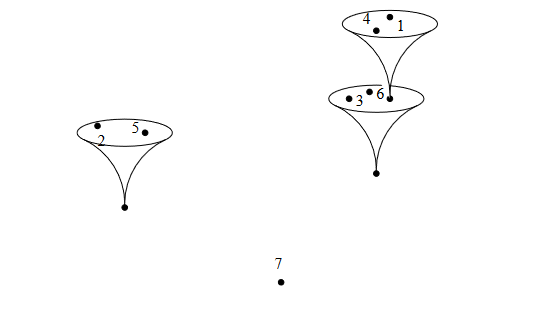
\includegraphics[width=0.8\textwidth]{img/sinha-fm-element}
    \caption{A point in $\Conf_M(6)$ associated to a tree with four internal nodes. }
\end{figure}    

\begin{definition}
    An $f$-tree is a rooted connected tree with labelled leaves and no bivalent internal vertices. The root is allowed to be bivalent (and also univalent).
    
    By defining a relation via edge contraction, one obtains a poset structure on the set of $f$-trees with $k$ leaves, denote this by $\Phi_k$.
\end{definition}
See figure~\ref{sinha-trees} for an example.

\begin{figure}[ht]
    \centering
    \begin{subfigure}[b]{0.45\textwidth}
        \centering
        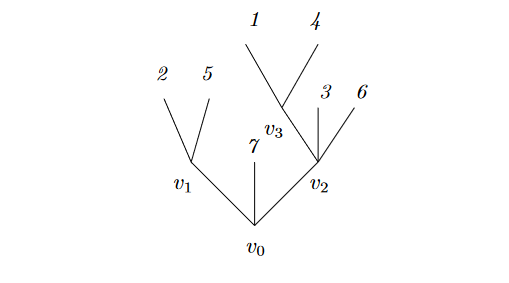
\includegraphics[width=\textwidth]{img/sinha-tree}
        \caption{An $f$-tree}
    \end{subfigure}
    \hfill
    \begin{subfigure}[b]{0.45\textwidth}
        \centering
        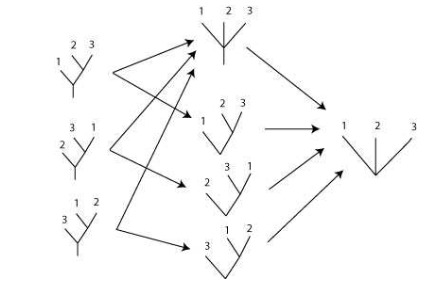
\includegraphics[width=\textwidth]{img/sinha-tree-poset}
        \caption{The poset $\Phi_3$ }
    \end{subfigure} 
    \caption{Example of $f$-trees. }\label{sinha-trees}
\end{figure}


\begin{theorem}
    There is a stratification on $\cConf_M(n)$ where each stratum $\cConf_M(T)$ corresponds to an $f$-tree $T$ and the poset of the stratification is $\Phi_n$. Similarly, for $\cConf_m(n)$, there is a stratification where each stratum $\cConf_m(T)$ corresponds to an $f$-tree $T$ where the root has degree at least $2$. 
\end{theorem}


\paragraph{Operad Structure on $\cConf_m(n)$} In the $M=\R^m$ case one may equip $\cConf_m(n)$ with an operad structure using the stratification explained earlier. 
\begin{theorem}
    The operad $\cConf_m$ is equivalent to the little $2$-disks operad $\mathcal D$.
\end{theorem}

To see this, we define a structure of an ``operad up to homotopy'' on $\Conf_n(m)$ (this is not standard terminology), in the sense that the associativity of composition does not hold on the nose, but there are canonical homotopies. There is then a zig-zag $\cConf_m \leftarrow \Conf_m \to \mathcal D_m$, where the first map preserves the operadic composition operations and is a homotopy equivalence on each level. The second map preserves the operadic composition operations up to homotopy and is also a homotopy equivalence on each level. This is enough to show that the homological operad structures agree, for an actual homotopy equivalence, one uses the Boardman-Vogt construction, which is a cofibrant resolution of topological operads.

To describe the operad structure ``up to homotopy'' on $\Conf_m$ in more detail, define a map $\Conf_m(n) \to \mathcal D_m(n)$ by drawing an outer disk around the barycenter of the configuration and drawing small disks around each point in the configuration (the radii should depend continuously on the configuration). Using this map and the projection to the center map $\mathcal D_m(n) \to \Conf_m(n)$, one may transfer the composition operations of $\mathcal D_m(n)$ to $\Conf_m(n)$. If multiple compositions in $\Conf_m$ are performed, the disks may differ in size, which leads to different configurations, but there is a homotopy comes from rescaling the circles. 

For the $m=2$ case one can alternatively apply a recognition principle by Fiedorowicz: The symmetric group acts freely on $\Conf_n(\R^2)$ and the quotient $\Conf_n(\R^2) / S_n = \UConf_n(\R^2)$ has $\pi_1(\UConf_n(\R^2)) = B_n$, the braid group of $n$ braids. The universal cover of $\Conf_n(\R^2)$ is contractible and has a braid operad structure with free action. Any two such operads with contractible total space and free group action are equivalent. Quotienting the equivalence by $PB_n = \ker(B_n \to S_n)$ we obtain an equivalence of the original operads. Then show that this also holds for $\cConf_n(\R^2)$.


\paragraph{Operadic module structure of $\Conf_M$} We build a fiberwise version of the configuration spaces $\cConf^M(n) = Fr_M\times_{SO(n)} \cConf_m(n)$, where $Fr_M$ is the oriented orthonormal frame bundle of some (irrelevant) metric on $M$. This is an operad in spaces over $M$. Then $\cConf_M$ is an operadic right module over $\cConf^M$. If $M$ is framed, then $\cConf_M$ is a module over the $\cConf(\R^D)$ operad.






\subsection{Graph Complex of Configuration Spaces}

\subsubsection{The case $M=\R^m$}

\paragraph{Homology} We first exhibit a homological complex construction; this is ad-hoc, not following any reference. Recall from earlier that the homology is given as an operad generated by a multiplication $\mu$ and a bracket operation $b$. To a rooted binary tree with labeled vertices one can assign an element of $H_*(\Conf_m(n))$ by putting $b$ at each of the inner vertices. To a collection of such rooted trees (a forest), one can assign an element of $H_*(\Conf_m(n))$ by multiplying the previous elements up. These elements generate the homology as a module. 

We now create an operad of chain complexes related to rooted trees $\mathcal{RT}$, by using the same generators $\mu$ and $b=b_2$ as before, but we add generators $b_k\in\mathcal{RT}(k)$, which corresponds to a corolla with $k$ incoming vertices. Compositions of the generators $b_k$ can be graphically depicted as rooted trees, now no longer binary. $\mu$ is still commutative and associative. I haven't figured out how the Poisson relation translates to the higher terms, thus the operad structure is somewhat unclear for forest-like elements. The differential is given by the dual of edge contraction modulo some symmetries, so that the differential of $b_3$ is the Jacobi element of $b_2$. There is an exact sequence $H_{k(m-1)-1}(\Conf_m(k), \partial\Conf_m(k)) \to H_{k(m-1)-2}(\partial\Conf_m(k)) \to H_{k(m-1)-2}(\Conf_m(k))$. The generator $b_k$ represents the fundamental class of $H_{k(m-1)-1}(\Conf_m(k), \partial\Conf_m(k))$.

\paragraph{Cohomology} We now outline the complex descibing the cohomology of $\Conf_m(n)$. For a detailed construction, see \cite[Chapter 6]{lambrechts2014formality}. Consider diagrams (graphs) $\Gamma$ with $n$ labeled ``exterior'' points and an arbitrary finite number of indistinguishable ``interior'' points. Define a graded vector space freely generated by these graphs, where the degree of a graph is 
\begin{align*}
    \deg \Gamma = \abs{E_\Gamma} \cdot (m-1) - \abs{I_\Gamma} \cdot m.
\end{align*} 
We omit some details here: to choose appropriate signs in the differential later, one has to induce orders on most of the data of the graphs and talk about loops, parallel edges etc. The differential is given by edge contraction for edges with at least one internal vertex. Admissible diagrams contain no loops, no double edges, no internal vertices of valence $\leq 2$ and each internal vertex is connected to some external vertex. 

The admissible diagrams form a graph complex $\coGraphs_m$ with differential given by edge contraction. They form a Hopf cooperad with multiplication given by union of graphs, identifying the external vertices by their labels, and cooperadic cocomposition is dual to the operad with operadic composition $\comp_i$ which inserts at the node $i$ a graph and sums over all choices of connecting the loose edges to $i$. 

\begin{theorem}
    The complex of admissible diagrams is quasi-isomorphic to the singular cochain complex of $\cConf$.
\end{theorem}

\paragraph{Graph Complex according to Idrissy \cite{idrissi2021real}} Assume $M$ is a simply connected compact manifold and $A$ a Poincaré duality model of $M$. The Lambrechts-Stanley model of $\Conf_m(r)$ is the chain complex 
\begin{align*}
    G_A(r) \defeq A^{r\otimes} \otimes S(\omega_{ij})_{1 \leq i\neq j\leq r} / I.
\end{align*}
where $I$ is generated by 
\begin{itemize}
    \item the relations $\omega_{ij}^2, \omega_{ji} = (-1)^m \omega_{ij}$, $\omega_{ij}\omega_{jk} + \omega_{jk}\omega_{ki} + \omega_{ki}\omega_{ij} = 0$ that appear in the presentation of the cohomology by Arnol'd.
    \item $p_i^*(a)\omega_{ij} = p_j^*\omega_{ij}$ for an $a\in A$ and $1\leq i\neq j \leq r$. 
\end{itemize}

Here, $p_{ij} \colon A\otimes A \to A^{\otimes r}$ is $p_{ij}^*(a\otimes b) = p_i^*(a)\cdot p_j^*(b)$ where $p_i^*\colon A\to A^{\otimes r}$
\begin{align*}
    p_i^*(a) \defeq 1\otimes \cdots \otimes 1\otimes a\otimes\cdots\otimes 1
\end{align*}
with the $a$ in the $i$-th position. 

The differential $d = d_A + d_{split}$ on $G_A(r)$ is the sum of the differential induced by that on $A$ and replacing an edge by the diagonal class of $A$
\begin{align*}
    d_{split}(\omega_{ij}) = p_{ij}^*(\Delta_A).
\end{align*}



\paragraph{Intuition} The following is not meant to be precisely true, but it still gives good intuition. Let $\Gamma$ be an admissible diagram with $\ell$ interior vertices and fix an order on the interior vertices. Consider the intersection $\bigcap \pi_{ij}^{-1}(c_{ij})\subset \cConf_m(n+l)$, where $c_{ij}$ are constants. This is a space with expected codimension $\abs{(E_\Gamma)}\cdot (m-1)$, we interpret it as a homology class in $H_*(\cConf_m(n+\ell), \partial\cConf_m(n+\ell))$. Map this along the projection $p_{n,\ell}\colon \cConf_m(n+\ell)/\partial\cConf_m(n+\ell) \to \cConf_m(n)/\partial\cConf_m(n)$ which forgets the last $\ell$ points, denote the resulting class by $a_\Gamma\in H_*(\cConf_m(n), \partial\cConf_m(n))$, now of expected codimension $\abs{(E_\Gamma)}\cdot (m-1) - \ell\cdot m$. The boundary of the space is given by edge contraction of $\Gamma$. Under Poincare duality, it corresponds to the form $\bigwedge \alpha_{ij}$ of degree $\abs{E_\Gamma}\cdot (m-1)$. 

For example, figure \ref{graph-complex-ex} shows how the Arnol'd identity $\alpha_{12}\alpha_{23} + \alpha_{23}\alpha_{31} + \alpha_{31}\alpha_{12} = 0$ in cohomology arises in this way: Interpret the diagram in (b) as the space of configurations of four points where the relative directions between the interior and the exterior point are fixed. The codimension one boundary of this is given by the configurations where the interior point is infinitesimally close to one of the three exterior points (and the relative directions are still fixed). Forgetting the interior point now yields three components as in (a).  

\begin{figure}[ht]
    \centering
    \begin{subfigure}[b]{0.65\textwidth}
        \centering
        \includesvg[width=\textwidth]{img/graph-complex-jacobi-2}
        \caption{The Arnol'd identity $\alpha_{12}\alpha_{23} + \alpha_{23}\alpha_{31} + \alpha_{31}\alpha_{12} = 0$}
    \end{subfigure}
    \hfill
    \begin{subfigure}[b]{0.3\textwidth}
        \centering
        \includesvg[width=\textwidth]{img/graph-complex-jacobi-1}
        \caption{A cochain whose boundary is the Arnol'd identity}
    \end{subfigure} 
    \caption{Arnol'd identity in the graph complex. }\label{graph-complex-ex}
\end{figure}

This intuition the definition of the boundary operator and the product structure. The operad structure is not immediately clear. 

Note that the projection $\cConf_m(n+\ell) \to \cConf_m(n)$ becomes an umkehr map in cohomology due to Poincare duality. Thus one can use fiber integration to represent this. The construction ``configuration space integral'' quasi-isomorphism $Graphs_m \to \Omega_{PA}(\cConf_m)$ essentially works as described above. The construction of the umkehr map is difficult, as the fiber is not a manifold, hence one uses PA forms here. 

\subsubsection{The case $M$ manifold}

Following \cite{campos2016model}. 

%\paragraph{Decorated Graphs} Let $H$ be a vector space and $S$ be a collection of graphs with vertex sets $V_G$ for $G\in S$. The vector space of decorated graphs is the space

%\begin{align*}
%    \bigoplus {G\in S} \Lambda(H_v \mid v\in V_G)
%\end{align*}

%where $\Lambda$ is the commutative algebra generated freely by the vector spaces and the $H_v$ are distinct copies of $H$ for each vertex $v$. Thus each vertex may be decorated with multiple elements of $H$ at each vertex, which are related tensorially. 

% \paragraph{Pre-dual graphs} Let $V$ be an $N$-dimensional graded vector space with a non-degenerate pairing of degree $-D$; $\langle\blank,\blank,\rangle\colon V\otimes V \to \R$ s.t. $\langle x, y\rangle = (-1)^{kl+d}\langle y, x\rangle$. The example to keep in mind is the cohomology of a connected $N$-manifold. We may require that the pairing is compatible with the multiplication or a differential. 

% Let $e_1, \dots, e_N$ be a basis of $V$. Denote by $\coGra_V(n)$ the free graded commutative algebra generated by symbols $s^{ij}$ of degree $D-1$ for $i,j \leq n$ and $e_1^j\dots e_N^j, j=1,\dots,n$, quotiented by $e^j_1 - 1$. Define a differential via 
% \begin{align*}
%     &de^j_\alpha = 0 \\
%     &ds^{ij} = \sum_{\alpha, \beta} g^{\alpha\beta}e^i_\alpha e^j_\beta
% \end{align*}
% where $g^{kl}$ is the inverse of the matrix describing the pairing on $V$ (so $\sum_{g^{\alpha, \beta}} e_\alpha e_\beta$ is the ``diagonal class'' i.e.\ the associated copairing). More abstractly, one can also present this without choosing a basis in $V$, by considering the graded commutative algebra generated by $n$ different copies of $V$ and the free symbols $s^{ij}$. A homogeneous element corresponds to a graph with $n$ vertices and decorations at each vertex with elements of $V$, see figure \ref{cw-graph-example}. 

If $M$ is a compact orientable manifold, denote by $\coGra_M(n) = \coGra_{H^*(M)}(n)$. If $M = \R^D$ and hence $V=k$ concentrated in degree $0$, then the above construction, omitting differentials, yields a graded vector space, which we denote $\coGra_D(n)$; this corresponds to undecorated differentials. 

$\coGra_D$ is a cooperad and $\coGra_M$ is a comodule of $\coGra_D$. 

\begin{figure}[ht]
    \centering
    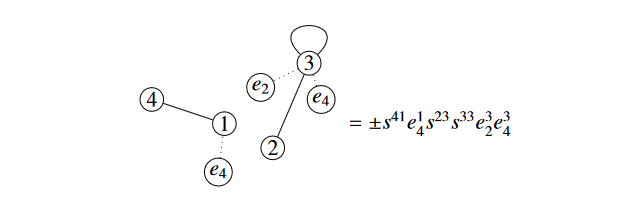
\includegraphics[width=0.8\textwidth]{img/campos-willacher-graph-dual-example.png}
    \caption{An example of a graph describing an element in $\coGra_V(4)$}\label{cw-graph-example}
\end{figure}

\paragraph{The dual graph complex $\coGraphs_M(n)$} As a vector space, it is spanned by $n$ labeled external vertices and an arbitrary finite number of internal vertices, decorated by (possibly multiple) cohomology classes of deg $\geq 1$, under the condition that there are no connected components without external vertices. There is a graded commutative algebra structure given by superposition of external vertices (i.e. disjoint union of graphs followed by identifying the external vertices with the same label). The differential splits as $\delta_{contr} + \delta_{cut} = \delta_{contr} + \Delta^* + \delta_{Z_M}$, where $\delta_{contr}$ contracts edges with at least one internal vertex and $\delta_{cut}$ splits edges with the copairing. This may produce ``forbidden'' graphs containing connected components without external vertices. This is the $\delta_{Z_M}$ part, which maps these components to a scalar via the function $Z_M$.

There is a similar construction for the $M=\R^D$ case for $\coGraphs_D(n)$, the difference is that all internal vertices of graphs are required to be at least trivalent (and no decorations are required). This has a cooperad structure which is induced by the dual of contracting a subgraph: for the coaction on a graph $\Gamma$ one sums over tuples $\Gamma', \Gamma_1, \dots, \Gamma_k)$ such that when each graph $\Gamma_i$ is inserted at the vertex $i$ of $\Gamma'$, one can reconnect the loose edges such that one obtains $\Gamma$.  

TODO: Image

\begin{theorem}
There is a quasi-isomorphism between $\coGraphs_D$ and $\Omega_{PA}(\cConf_D)$ (which is equivalent to $\mathcal A_{PL}(\cConf_D)$), which is compatible with the cooperad structures (in an appropriate sense).

There is an equivalence between $\coGraphs_M$ and $\mathcal A_{PL}(\cConf_M)$ which is compatible with the cooperadic comodule structure. 
\end{theorem}

\begin{figure}[ht]
    \centering
    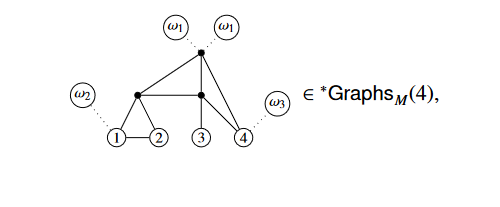
\includegraphics[width=0.5\textwidth]{img/cw-graphs-ast-example.png}
    \caption{An example element of $\coGraphs_V(4)$}\label{cw-graphs-ast-example.png}
\end{figure}    
\begin{figure}[ht]
    \centering
    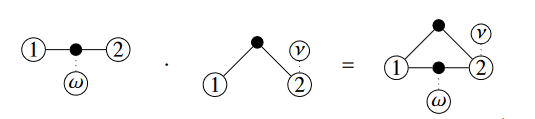
\includegraphics[width=0.7\textwidth]{img/cw-graphs-mult.png}
    \caption{An example element of $\coGraphs_V(4)$}\label{cw-graphs-mult}
\end{figure}















\section{String Topology Operations via Configuration Spaces}

In this section we construct the string product and coproduct in the form that they will be used later. We use a slightly unusual construction using configuration spaces instead of the usual construction using Pontrjagin-Thom collapse maps. We begin with the construction of the intersection product on a closed manifold $M$ using configuration spaces. We then give an analogous construction of the string product and coproduct. 

Let $M$ be a closed oriented manifold. Recall $\cConf_M(2)$ is the compactified ordered configuration space of two points in $M$. This is a stratified manifold with a substratum diffeomorphic to the unit sphere bundle $UTM\subset TM$. The square
\begin{equation}\label{M_pushout}
\begin{tikzcd}
    UTM \dar\rar & \cConf_M(2)\dar \\
    M \rar["\Delta"] & M\times M
\end{tikzcd}
\end{equation}
is a homotopy pushout since it is a pushout of topological spaces and map $UTM \to \cConf_M(2)$ is a cofibration. Thus the homotopy cofibers of the  vertical maps are homotopy equivalent due to the pasting law for homotopy pushouts %TODO reference
and they are in fact versions of the Thom space $DM / UTM$ (where $DM$ is the unit disk bundle). This is the main ingredient to the construction of the intersection product. 

\begin{lemma}\label{lemma_pullback_cube}
    Let $E\to M\times M$ be a fibration and $E|_M, E|_{UTM}, E|_{\cConf_M(2)}$ the pullbacks of $E\to M\times M$ along the maps in diagram \ref{M_pushout}. Then

    \begin{equation} \label{E_pushout}
    \begin{tikzcd}
        E|_{UTM} \dar\rar & E|_{\cConf_M(2)}\dar \\
        E|_{M} \rar["\Delta"] & E
    \end{tikzcd}
    \end{equation}
    
    is a homotopy pushout. In particular the cofibers are equivalent.    
\end{lemma}
This follows from Mather's cube theorem, where diagram~\ref{M_pushout} is the bottom face of the cube, diagram~\ref{E_pushout} is the top face, and the side faces are pullbacks by construction. %TODO reference here


\subsection{Intersection Map in $M$ via Configuration Spaces}\label{subsec:intersection-in-M-via-conf}

We want to construct the intersection product map $H_*(M) \otimes H_*(M) \to H_{*-n}(M)$. In cohomology, this corresponds to a map $H^*(M) \otimes H^*(M) \from H^{*-n}(M)$. For a review of the intersection product, see section \ref{sec:intersection_product}.

Using the observations from above, we can construct the intersection coproduct as the sequence of maps
\begin{equation}
\begin{tikzcd}
    H^*(M\times M) & \lar H^*(M\times M, \cConf_M(2)) \dar["\iso"] & \ \\
    & H^*(M, UTM)& \lar["\cupp Th"] H^{*-n}(M)
\end{tikzcd}
\end{equation}
The cohomologies in the middle of the diagram are the cohomologies of the mapping cone, hence of the homotopy cofiber. The vertical map is the isomorphism from above. The last arrow is the Thom isomorphism, i.e.\ multiplication with the Thom class, which is a cohomology class of the Thom space which represents the orientation of $M$. % TODO: Reference for Thom Iso

\begin{theorem}
    The above map is identical to the intersection product defined via Poincaré Duality in section \ref{sec:intersection_product}. 
\end{theorem}
\begin{proof}
    We show this for the homological version of the intersection product, the cohomological statement is analogous. The homological version of the above construction is
    \begin{equation}
        \begin{tikzcd}
            H_*(M\times M) \rar & H_*(M\times M, \cConf_M(2)) &  \\
            & \uar["\iso"] H_*(M, UTM) \rar["\capp Th"]&  H_{*-n}(M)
        \end{tikzcd}
    \end{equation}
    In the proof of theorem \ref{thm:intersection_product_tubular} it is shown that the intersection product is equal to the sequence 
    \begin{align*}
        H_*(M\times M)\xrightarrow{\capp u_\Delta} H_{*-n}(M\times M) \xrightarrow{\pi_{1*}} H_{*-n}(M)
    \end{align*}
    The first map is the cap product with $u_\Delta\in H^n(M\times M)$, the Poincaré dual of the diagonal $\Delta_*[M]\in H_*(M\times M)$. By the arguments in the referenced subsection, this is equivalent to taking the intersection product with the diagonal class $\Delta_* [M]$. The second map is induced by the projection to the first factor $M\times M\to M$.

    Let $u\in H_n(M, UTM)$ be the Thom class of the tangent bundle of $M$, it is shown in theorem \ref{thm:thom_class_dual} that this is Poincaré dual to the zero section of the unit disk bundle of $TM$. Denote by $u_\Delta^c$ its image under the isomorphism $H_*(M\times M, \cConf_M(2)) \iso H_*(M, UTM)$. 
    
    We consider the following diagram. 
    \begin{center}
        \begin{tikzcd}
            H_*(M\times M) \dar["\capp u_\Delta"] \rar & H_*(M\times M, \cConf_M(2)) \dar["\capp u_\Delta^c"] & \lar["\iso"] H_*(M, UTM) \dar["\capp u"] \\
            H_{*-n}(M\times M) \dar["\pi_{1*}"] \rar & H_{*-n}(M\times M) \dar["\pi_{1*}"] & \lar["\Delta"] H_{*-n}(M) \dar \\
            H_{*-n}(M) \rar["\id"] & H_{*-n}(M) & \lar["\id"] H_{*-n}(M)
        \end{tikzcd}
    \end{center}
    
    Commutativity of the outer square implies our result that the two versions of the intersection product are identical. It is clear that all squares except for the upper left commute. 

    To show that the upper left square commutes, we need to show the following claim: the restriction $r\colon H^n(M\times M, \cConf_M(2)) \to H^n(M\times M)$ maps $u_\Delta^c$ to $u_\Delta$. To do so, we retrace the proof of lemma 4.2 in \cite{hutchings2011cup}. The claim is equivalent to $\Delta_*[M] = [M\times M]\capp r(u^c_\Delta) \in H^n(M\times M)$. To show this, consider the following diagram
    \begin{center}
        \begin{tikzcd}
            H_{2n}(M\times M) \otimes H^n(M\times M, \cConf_M(2)) \dar \rar & H_{2n}(M\times M) \otimes H^n(M\times M) \dar["\capp"] \\
            H_{2n}(M\times M, \cConf_M(2))\otimes H^n(M\times M, \cConf_M(2)) \rar["\capp"] \dar["\iso"] & H_n(M\times M) \\
            H_{2n}(M, UTM)\otimes H^n(M, UTM) \rar["\capp"] \dar["\iso"] & H_n(M) \uar \\
            H_{2n}(DTM, UTM)\otimes H^n(DTM, UTM) \arrow[ur, "\capp"] &
        \end{tikzcd}
    \end{center}
    The lower and center left maps are the tensor product of two isomorphisms. The commutativity of the diagram is due to the naturality of the cap product. Now we chase $[M\times M]\otimes u_\Delta^c$ through the diagram, starting in the upper left and ending in the center right. The path through the top right maps it to $[M\times M]\capp r(u_\Delta^c)$. The fundamental class $[M\times M]$ is mapped via $H_2n(M\times M)\to H_{2n}(M\times M, \cConf_M(2))\to H_{2n}(M, UTM) \iso H_{2n}(DTM, UTM)$ to the fundamental class $[DTM]$. TODO: Actually give a proof of this.
    
    Thus $[M\times M]\otimes u_\Delta^c$ is mapped to $[DTM] \otimes u$. By theorem \ref{thm:thom_class_dual}, $[DTM] \capp u = [M]$ and we have shown $\Delta_*[M] = [M\times M]\capp r(u^c_\Delta)$. This shows the claim and hence concludes the proof.
\end{proof}


In comparison to the construction via tubular neighborhoods, which requires a choice of tubular neighborhood, this construction only requires a choice of equivalence between the cofibers of diagram~\ref{M_pushout}
\nocite{*} (and a construction of the unit tangent bundle).

\subsection{String Product (cohomology coproduct)}
The free loop space $LM$ is the pullback of the path space fibration $PM \to M\times M$ and the diagonal map $M\to M\times M$. As the first map is a fibration, this is in fact a homotopy pullback. %TODO Reference

By applying lemma \ref{lemma_pullback_cube} to the fibration $LM\times LM\to M\times M$, we obtain the following homotopy pushout diagram:
\begin{equation}
    \begin{tikzcd}
        LM\times LM|_{UTM} \rar\dar & LM\times LM |_{\cConf_M(2)} \dar \\
        LM\times LM|_M \rar & LM\times LM
    \end{tikzcd}
\end{equation}
where each term is the fiber product of $LM\times LM$ with the corresponding term in~\ref{M_pushout} over $M\times M$. Thus $LM\times LM|_M$ is the space of figure eights in $M$, i.e.\ two loops starting at the same point in $M$. $LM\times LM|_{UTM} = (LM\times LM)\times_{M\times M} UTM$ is the space of figure eights in $M$, together with a unit tangent vector at the node of the eight. $LM\times LM|_{\cConf_M(2)}$ is a space which contains pairs of loops which need not necessarily intersect, but if they intersect at $t=0$, then we additionally have a unit tangent vector at the node. 

Thus we can define a lifting of the intersection map:
\begin{equation}
    \begin{tikzcd}
        H^{*}(LM \times LM) & \lar H^*(LM\times LM, LM\times LM|_{\cConf_M(2)}) \dar["\iso"] & &\\
        & H^*(LM\times LM|_{M}, LM\times LM|_{UTM}) & \lar["\cupp Th"] H^{*-n}(LM\times LM|_M)
    \end{tikzcd}
\end{equation}
The map $H^*(LM\times LM|_{UTM}, LM\times LM|_M) \xleftarrow{"\cupp Th"} H^{*-n}(LM\times LM|_M)$ is given by taking the cup product with the pullback of the Thom class of $M$ along the map of pairs $(LM\times LM|_{M}, LM\times LM|_{UTM}) \to (M, UTM)$. The vertical map comes from the isomorphism of the cofibers. 

The string product is now the following map: 
\begin{align*}
    H^*(LM)\otimes H^*(LM) \from H^*(LM\times LM) \from H^{*-n}(LM\times LM|_M) \from H^{*-n}(LM),
\end{align*}
here the last map is induced by the map $LM\times LM|_M \to LM$, which is given by concatenation of loops with shared base point.

\subsection{String Coproduct (Cohomological Product)}

The coproduct is going to be defined relative to constant loops, i.e.
\begin{align*}
    H^*(LM, M) \from H^*(LM, M)\otimes H^*(LM, M)[n-1]
\end{align*}
where the $[n-1]$ denotes a shift of the index of the graded vector space by $n-1$. 

\paragraph{Splitting/Reparametrization Map} In place of the concatenation map in the previous subsection, we use here the splitting / reparametrization map, which will be a map on cohomology
\begin{align*}
    s^*\colon H^{*}(LM, M) \from H^{*+1}(\Map(\ocircle_2), LM\coprod_M LM),
\end{align*}
where $\Map(\ocircle_2, M) = \Map(\ocircle_2)$ is the space of loops in $M$ with two marked points at $t=0$ and $t=\frac 12$ (formally this is identical with $LM$, but there is a fibration $\Map(\ocircle_2, M)\to M\times M$) and $LM\coprod_M LM$ is the subspace of $\Map(\ocircle_2)$ such that one of the two paths is constant. This map can be thought of as mapping a loop $\gamma$ to the $t$-indexed family of path pairs $(\widehat{\gamma|_{[0, t]}}, \widehat{\gamma|_{[t, 1]}})$, where the hat represents a reparametrization of the paths. 

In more detail, let $s$ be the map 
\begin{align*}
    s\colon I\times LM & \to\Map(\ocircle_2),\\
    (t, \gamma) &\mapsto s\mapsto \begin{cases}
        \gamma(2 st) & \text{if}\ 0 \leq s \leq \frac 12\\
        \gamma(2t(1-s)+2(s-\frac 12))& \frac 12\leq s \leq 1
    \end{cases}
\end{align*}
which splits the loop into the parts defined on the intervals $[0, t]$ and $[t, 1]$ and reparametrizes so they are defined on $[0, \frac 12]$ and $[\frac 12, 1]$ respectively. This is a map of pairs
\begin{align*}
    s\colon (I\times LM, \partial I\times LM \union I\times M) \to (\Map(\ocircle_2, M), LM\coprod_M LM).
\end{align*} 
By taking the product with (a representative of) the fundamental class of $S^1$, we obtain a suspension map on (e.g.\ singular) chains $ C_{*}(LM, M) \to C_{*+1}(I\times LM, \partial I \times LM \union I\times M)$ and composing its dual on cohomology with the previous map yields a map 
\begin{align*}
    s^*\colon H^{*}(LM, M) \from H^{*+1}(I\times LM, \partial I \times LM \union I\times M) \from H^{*+1}(\Map(\ocircle_2), LM\coprod_M LM)
\end{align*}
which is the map we intended to construct.

\paragraph{Intersection map} 
As the next step of the construction, we need an intersection map, which in homology can be thought of as intersecting a homology class in $\Map(\ocircle_2, M)$ with $\Map(8, M) \subset \Map(\ocircle_2, M)$. As we are still working with relative cohomology, this will be a map
\begin{align*}
    H^{*+n}(\Map(\ocircle_2, M), LM\coprod_M LM) \from H^*(\Map(8, M), LM \coprod_M LM)
\end{align*}

We apply \ref{lemma_pullback_cube} to the fibration $\Map(\ocircle_2)\to M\times M$. Thus we obtain the homotopy pushout

\begin{equation}
    \begin{tikzcd}
        \Map'(8) \rar\dar &\Map'(\ocircle_2)\dar \\
        \Map(8) \rar & \Map(\ocircle_2)
    \end{tikzcd}
\end{equation}

where $\Map(8, M)$ consists of figure eight loops in $M$ and $\Map(\ocircle_2)$ consists of loops with an additional marked point, and in $\Map'(8)$ we again have an additional unit tangent vector at the node of the figure eight. We have again have an equivalence of cofibers $\Map(8) / \Map'(8) \iso \Map(\ocircle_2)/\Map'(\ocircle_2)$, and hence an equivalence of cofibers of cofibers
\begin{align*}
    \frac{\Map(\ocircle_2,M) / \Map'(\ocircle_2, M)} {(LM \coprod_M LM) } \iso \frac{(\Map(8,M) / \Map'(8, M)) }{(LM \coprod_M LM)}
\end{align*}

We now have a sequence of maps 
\begin{align*}
    H^*(\Map(\ocircle_2), LM\coprod_M LM) \from H^*(\Map(\ocircle_2)/ \Map'(\ocircle_2), LM\coprod_M LM) \\ \iso H^*(\Map(8) / \Map'(8), LM \coprod_M LM) \from H^{*-n}(\Map(8), LM \coprod_M LM)
\end{align*}
The last map is the cup product with the pullback of the Thom class $\tau\in H^n(M, UTM)$ along the map $H^*(\Map(8), \Map'(8)) \from H^*(M, UTM)$.

\paragraph{Definition of the string coproduct} Taking the two maps constructed in the previous paragraphs together, we get the coproduct:
\begin{align*}
    H^*(LM, M) \from H^{*+1}(\Map(\ocircle_2), LM \coprod_M LM) \\
    \from H^{*+1-n}(\Map(8), LM\coprod_M LM) \from H^*(LM, M)^{\otimes 2}[n-1]
\end{align*}
where the last map is induced by the inclusion $\Map(8)\to LM\times LM$.

\paragraph{The case $\chi(M) = 0$} We assume that $M$ has trivial Euler characteristic. Recall that the Thom class of $M$ maps to the Euler class under the sequence $H^n(DTM, UTM)\to H^n(DTM)\iso H^n(M)$ and hence if the Euler class is $0$, the Thom class is the coboundary of some class in $H^{n-1}(TM_0)\iso H^{n-1}(UTM)$.

The splitting / reparametrization map is obtained via the same formula as before, but it is now a map $H^*(LM) \from H^{*+1}(\Map(\ocircle_2), \Map(8))$. The intersection map is now a map $H^*(\Map(\ocircle_2), \Map(8)) \from H^{*-n}(\Map(8))$, which is given as the sequence of maps
\begin{align*}
    H^*(\Map(\ocircle_2), \Map(8)) \\ \from H^*(\Map'(\ocircle_2), \Map'(8)) \xleftarrow{\delta} H^{*-1}(\Map'(8)) \from H^{*-n-1}(\Map(8))
\end{align*}


\subsection{Exercises}

\begin{enumerate}
\item Show the pasting lemma: Given a diagram as follows, if the right square is a (homotopy) pullback, then the total square is a (homotopy) pullback if and only if the left square is a pullback. Similarly if the left square is a (homotopy) pushout, then the total square is a (homotopy) pushout if and only if the right square is a (homotopy) pushout.
\begin{equation}
    \begin{tikzcd}
        A \dar\rar & B \dar\rar &\dar C \\
        D \rar & E \rar & E 
    \end{tikzcd}
\end{equation}

\item Show that relative homology computes the homology of the cofiber, that is if $A\injto B$ is a cofibration, then $H(B/A) \iso H(B, A)$.

\item Show Mather's cube theorem for regular and for homotopy pullbacks and pushouts. 

\item Show that the following definitions of the intersection map for the string product are equivalent:
\begin{enumerate}
    \item The definition given earlier
    \begin{equation}
        \begin{tikzcd}
            H^{*}(LM \times LM) & \lar H^*(LM\times LM, LM\times LM|_{\cConf_M(2)}) \dar["\iso"] & &\\
            & H^*(LM\times LM|_{M}, LM\times LM|_{UTM}) & \lar["\cupp Th"] H^{*-n}(LM\times LM|_M)
        \end{tikzcd}
    \end{equation}
    \item The following definition from \cite{cohen2002homotopy}: Let $\nu(\Delta)$ be a tubular neighborhood of the diagonal $\Delta\colon M \to M\times M$ and $\nu(\tilde\Delta) = ev^{-1}(\nu(\Delta))$ the pullback along the evaluation $ev\colon LM\times LM\to M\times M$, which is an open neighborhood of the embedding $\tilde\Delta\colon LM\times_M LM\injto LM\times LM$. This neighborhood is homotopy equivalent to the total space of the pullback bundle $ev^*(\nu(\Delta)) = ev^*(TM)$. The intersection map is defined as the composition
    \begin{align*}
        H^*(LM\times LM) \from H^*(LM\times LM, LM\times_M LM) \iso H^*(\nu(\tilde\Delta), \nu(\tilde\Delta)_0) \\ 
        \iso H^* (ev^*(TM), ev^*(TM)_0) \from H^{*+d}(\nu(\tilde\Delta)) \from H^{*-n}(LM\times_M LM)
    \end{align*}
    where the last map is the Thom isomorphism of the $n$-dimensional bundle $ev^*(TM)$ over $LM\times_M LM$.
\end{enumerate}

\item What is the definition of $ES^1$? Why is $LM\times_{S^1} ES^1$ the homotopy quotient of the group action? Are $LM/S^1$ and the homotopy quotient $LM\times_{S^1} ES^1$ homotopy equivalent in this case?


\end{enumerate} % End Exercises













\newpage
\appendix
\section{Thom Isomorphism and Poincaré Duality}
We state some classical results relating to the Thom Isomorphism theorem and Poincaré Duality. We use homology with $\Z$-coefficients throughout, but other coefficient systems may be used, if the definition of orientation is adjusted correspondingly.


\subsection{Poincaré Duality}
Let $M$ be a compact orientable manifold of dimension $n$ with boundary $\partial M$. Since $M$ is oriented, one can assign to any $p\in M\setminus \partial M$ canonically a homology class $z_p\in H_n(M, M\setminus \{p\})$ which describes the orientation at $p$.
\begin{theorem} \label{thm:poincare_duality}
\begin{enumerate}[(a)]
    \item There exists a \emph{fundamental class} $[M]\in H_n(M,\partial M)$, such that for any $p\in M\setminus \partial M$, we have $[M]|_{(M, M\setminus\{p\})} = z_p\in H_n(U, U\setminus \{p\})$.
    \item If $\partial M = A \union B$ is the union of two compact $(n-1)$-dimensional manifolds with common boundary $\partial A = \partial B = A\isect B$, then the cap product with $[M]$ gives an isomorphism
    \begin{align*}
        H^k(M, A) \to H_{n-k}(M, B).
    \end{align*}
    \item In particular, there are isomorphisms
    \begin{align*}
        H^k(M) \to H_{n-k}(M, \partial M) \\
        H^k(M,\partial M) \to H_{n-k}(M).
    \end{align*}
\end{enumerate}
\end{theorem}

This is \cite[Thm 3.43]{hatcher2002algebraic} and the surrounding material.

\subsection{Thom Isomorphism}
Let $\xi$ be a rank $n$ vector bundle $E\xrightarrow{\pi} B$ and let $E_0$ be $E$ minus the zero section. Let $UE\to DE$ be the inclusion of the unit sphere bundle of $E$ into its unit disk bundle, then the homotopy cofibers of $UE\to DE$ and $E_0\to E$ are homotopy equivalent and the space $Th(\xi) = DE / UE$ is called the Thom space of $\xi$. 

If $\xi$ is oriented, one can assign canonically to every fiber $F=\pi^{-1}(b)$ a cohomology class $u_F\in H^n(F, F_0)$, such that the assignments are locally compatible.

\begin{theorem}
    Let $\xi$ be an oriented rank $n$ vector bundle with paracompact base space.
    \begin{enumerate}[(a)]
        \item There exists a unique cohomology class $u=u(\xi)\in H^n(E, E_0)$ such that $u|_F = u_F\in H^n(F, F_0)$. This is called the \emph{Thom class} or fundamental class of $\xi$.
        \item The following map is an isomorphism
        \begin{align*}
            y \mapsto y\cupp u, \quad H^*(E) \to H^{n+*}(E, E_0)    
        \end{align*}
        \item The following map is an isomorphism
        \begin{align*}
            \eta \mapsto \eta\capp u, \quad H_{*+n}(E, E_0) \to H^{*}(E)
        \end{align*}
    \end{enumerate}
\end{theorem}

The \emph{Thom isomorphism} is one of the following compositions of isomorphisms
\begin{align*}
    \Phi^*\colon H^*(B)\xrightarrow{\pi^*}H^*(E)\xrightarrow{\cupp u}H^{*+n}(E, E_0) \\
    \Phi^*\colon H_{*+n}(E, E_0) \xrightarrow{\capp u} H_*(E)\xrightarrow{\pi_*}H_*(B)
\end{align*}

For a detailed proof, see \cite{milnor1974characteristic}. We give a quick sketch of the proof there. One first verifies that the theorem holds for trivial vector bundles, i.e.\ cross products. Using a Mayer-Vietoris argument one then shows that it holds on finite unions of trivialization domains, in particular on compact base spaces. For the general cases, one uses that homology is a colimit indexed by compact spaces.

There is an interpretation of the homological Thom isomorphism as taking the intersection with the zero section. We state this cleanly in \ref{thm:thom_iso_intersection} after introducing umkehr maps. This is a consequence of the following. 

\begin{theorem}\label{thm:thom_class_dual}
    Let $E\to M$ be a smooth orientable rank $r$ vector bundle over a compact orientable manifold with boundary $\partial M$. Then the Thom class $u=u(E)\in H^r(E, E_0)$ is Poincare dual to the zero section of $E$: After choosing a metric, let $DE$ and $SE$ be the unit ball resp.\ sphere bundles of $E$ and $[DE]\in H^{r+n}(DE, SE)$ the fundamental class, then
    \begin{align*}
        [DE] \capp u = [M]\in H_n(DE)
    \end{align*}
\end{theorem}

\begin{proof}[Proof Sketch]
    In a trivialization domain $U$, one has $E|_U = U \times \R^r$ and the orientation classes are given as follows. The restriction of $u$ to $(E|_U, E_0|_U)$ is the pullback of a class in the fiber direction: $u|_U = \pi_{D^r}^{*}\left(u_{(D^r, S^{r-1})}\right)\in H^*(E|_U, E_0|_U)$, for some $u_{(D^r, S^{r-1})}\in H^*(D^r, S^{r-1})$. The fundamental class $[DE]$ is locally a cross product: at any $p\in U$, one has $[DE]|_{(DE|_U, DE|_{U\setminus\{p\}})} = [M]|_{(U, U\setminus\{p\})} \times [D^r] \in H^*(E|_U, E|_{U\setminus\{p\}} \union E_0|_{U})$. Thus $[DE]|_{(DE|_U, DE|_{U\setminus\{p\}})} \capp u|_U = [M]|_{(U, U\setminus\{p\})}$.
\end{proof}

For an alternative proof, this is lemma 4.1 in \cite{hutchings2011cup}. 


\subsection{Euler Class}\label{subsec:euler_class}
\begin{definition}
    Let $\xi$ be an oriented rank $r$ vector bundle. The Euler class $e(\xi)\in H^r(B)$ of $\xi$ is image of the Thom class $u\in H^r(E, E_0)$ under the composition of maps $H^r(E, E_0)\to H^r(E)\xleftarrow{\iso} H^r(B)$.
\end{definition}
Equivalently, the Euler class is the class that corresponds to $u\cupp u$ under the Thom isomorphism, since $\phi(e) = p^*(e) \cupp u = j^*(u)\cupp u = u\cupp u$, for $p\colon E\to B$ and $j^*\colon H^*(E, E_0) \to H^*(E)$. 
\begin{theorem}\label{thm:euler_class}
    If $M$ is a smooth closed orientable manifold of dimension $n$ and $\xi=TM$ is its tangent bundle, then its Euler characteristic is 
    \begin{align*}
        \chi(M) = \langle e(TM), [M]\rangle.
    \end{align*}
    More generally, under the hypotheses of \ref{thm:thom_class_dual}, letting $s\colon B\to E$ be a section, the Euler class is Poincaré dual to the intersection $p_*(s_*[B]\capp s_*[B])\in H^{n-r}(B)$ of two sections in $E$.
\end{theorem}

The second part is \cite[Thm 5.2]{hutchings2011cup}.
In \cite{milnor1974characteristic}, the first part is shown for $\xi=TM$ using Poincaré duality. In \cite{hutchings2011cup}, the first part is concluded from the second using the Lefschetz fixed point theorem.

As a consequence of the theorem, the Euler class vanishes if and only if the Euler characteristic vanishes, and this is equivalent to the Thom class $u$ having a preimage wrt.\ the map $H^{r-1}(TM_0) \to H^r(TM, TM_0)$.

\subsection{Gysin Sequence}\label{subsec:gysin_sequence}
We follow \cite[pp. 438]{hatcher2002algebraic}. We consider fiber bundles with spherical fiber $S^{r-1}\to E\xrightarrow{p} B$. The Gysin sequence is an exact sequence of the form 
\begin{align*}
    \dots \to H^{i-n}(B) \xrightarrow{\cupp e} H^i(B) \xrightarrow{p^*} H^i(E) \to H^{i-n+1}(B)\to \dots
\end{align*}

One can associate to this sphere bundle an $r$-disk bundle using the mapping  cylinder $M_p$ of $p$. The mapping cylinder $M_p$ of a general continuous map is constructed as $M_p = (([0, 1]\times E) \coprod B) / (0, x) \sim p(x)$. Through the mapping cylinder, the map $p$ is factored into a cofibration and a surjective homotopy equivalence $E \injto M_p \surjto B$. Here, $E$ is included via $x\mapsto (1, x)$. 

In the special case where $p$ is the projection of a sphere bundle, the mapping cylinder of the projection map is a disk bundle $D^r\to M_p \to B$ with $E$ as its boundary sphere bundle. Assume for the moment that this bundle is orientable, so a Thom class $u\in H^r(M_p, E)$ exists. This is the case for example if $E$ is orientable. TODO: Why? / Do we need this?

We have the following commutative diagram: 

\begin{tikzcd}
    \dots \rar & H^i(M_p, E) \rar["j^*"] & H^i(M_p) \rar & H^i(E) \rar & H^{i+1}(M_p, E) \rar  &\dots \\
    \dots \rar & H^{i-r}(B) \uar["\Phi"][swap]{\iso}\rar["\cupp e"] & H^i(B)  \uar["p^*"][swap]{\iso} \rar["p^*"] & H^i(E) \uar["\id"]\rar & H^{i-r+1}(B) \uar["\Phi"][swap]{\iso} \rar  &\dots
\end{tikzcd}

Here $\Phi$ is the Thom isomorphism of the disk bundle $M_p\to B$, $e$ is the Euler class of $M_p$ and the vertical $p^*$ is an isomorphism as $M_p$ deformation retracts onto $B$. The square containing the map $\cupp e$ commutes due to the following: since $p^*(e) = j^*(c)$ by the definition of the Euler class, we can compute for $b\in H^{i-r}(B)$ that $j^*\Phi(b) = j^*(p^*(b)\cup u) = p^*(b) \cupp j^*(c) = p^*(b) \cupp p^*(e) = p^*(b\cupp e)$. 

Since the upper sequence is exact, so is the lower sequence.

\begin{theorem}
    Let $S^{r-1} \to E \xrightarrow{p} B$ be a fiber bundle over a paracompact base space, such that the associated disk bundle is orientable, denote by $e\in H^r(B)$ the Euler class of this disk bundle. The \emph{Gysin sequence} is the following exact sequence
    \begin{align*}
        \dots \to H_{i-r+1}(B) \to H_i(E) \xrightarrow{p_*} H_i(B) \xrightarrow{\capp e} H_{i-r}(B) \to \dots
    \end{align*}
    and in cohomology
    \begin{align*}
        \dots \to H^{i-r}(B) \xrightarrow{\cupp e} H^i(B) \xrightarrow{p^*} H^i(E) \to H^{i-r+1}(B)\to \dots
    \end{align*}
    The unlabeled map is $H_{i-r+1}(B) \xrightarrow{\Phi^{-1}} H_{i+1}(M_p, E) \xrightarrow{\partial} H_i(E)$. In the cohomology version, it is $H^i(E) \xrightarrow{\delta} H^{i+1}(M_p, E) \xrightarrow{\Phi^{-1}} H^{i-r+1}(B)$. 
\end{theorem}

We have shown the exactness of the sequence in cohomology, the sequence in homology is analogous. 

One can show that if $E$ is a smooth bundle over a smooth manifold $B$ then the map $H_{i-r+1}(B) \xrightarrow{\Phi^{-1}} H_{i+1}(M_p, E) \xrightarrow{\partial} H_i(E)$ is in fact the umkehr map $\pi_!\colon H_{i-r+1}(B) \to H_i(E)$. 

Recall from \ref{subsec:euler_class} that the Euler class is Poincaré dual a certain homology class, namely a class obtained by intersecting two sections in $M_p$, so the map $\capp e$ is the same as taking the intersection product with such a homology class. 

\section{Intersection Product and Umkehr Maps for Poincaré Duality Spaces}\label{sec:intersection_product}

Let $M$ be a smooth closed orientable $m$-dimensional manifold. Then the intersection product on the homology of $M$ is a map
\begin{align*}
    H_*(M) \otimes H_*(M) \to H_{*-m}(M)
\end{align*}
There is also a cohomology version is a map $H^*(M) \otimes H^*(M) \from H^{*-m}(M)$. We define the product using Poincaré duality and show that there is an equivalent definition via the Thom isomorphism. In the investigation of the intersection product we use umkehr maps: to a map $f\colon M\to N$ between poincaré duality spaces one can assign an umkehr map $f^!\colon H_*(N)\to H_{*+m-n}(M)$ in homology. The intersection product can be interpreted as the umkehr map associated to the diagonal $M\to M\times M$. 

\subsection{Intersection Product via Poincaré Duality} \label{subsec:intersection_product_via_pd}
\begin{definition}
The intersection product is the Poincaré dual of the cup product. Thus it is the upper map in the following commutative square, where the vertical maps are given by Poincaré duality and the lower map is the cup product.
\begin{equation}
    \begin{tikzcd}
        H_*(M) \otimes H_*(M) \dar["\iso"] \rar & H_{*-m}(M) \dar["\iso"] \\
        H^{m-*}(M)\otimes H^{m-*}(M) \rar["\cup"] &  H^{2m-*}(M)
    \end{tikzcd}
\end{equation}
\end{definition}
\begin{remark}
Since under the isomorphism $H_*(M\times M) \iso H_*(M)\otimes H_*(M)$, the cup product corresponds to the diagonal map, one can equivalently use the following diagram
\begin{equation}
    \begin{tikzcd}
        H_*(M\times M) \dar["\iso"] \rar & H_{*-m}(M) \dar["\iso"] \\
        H^{2m-*}(M\times M) \rar["\Delta^*"] & H^{2m-*}(M)
    \end{tikzcd}
\end{equation}
where the left vertical morphism is the Poincaré Duality of $M\times M$.
\end{remark}

\begin{remark}
The cap product and intersection product are related as follows: assume that $a\in H_i(M)$ and $\alpha\in H^{m-i}(M)$ are Poincaré dual to each other, so $[M]\capp \alpha = a = [M]\capp a$, then for any $b\in H_j(M)$, we can show 
\begin{align*}
    b\capp a = b\capp \alpha 
\end{align*}
Denote by $\beta$ be the Poincaré dual of $b$. The Poincaré dual of  $b\capp a = ([M]\capp \beta) \capp ([M] \capp\alpha)$ is $\beta\cupp\alpha$, hence $b\capp a = [M] \capp (\beta\cupp \alpha) = ([M]\capp \beta) \capp \alpha =  b\capp \alpha$.
\end{remark}

\subsection{Umkehr Maps via Poincaré Duality} \label{subsubsec:umkehr_maps_via_pd}
TODO: Bredon uses lower shrieks for the maps in homology, maybe we should too? 

There is a generalization of the intersection product, where the diagonal map is replaced with any continuous map between Poincaré duality spaces. 

\begin{definition}
Let $f\colon M\to  N$ be a map of smooth closed oriented manifolds. Then there is a contravariant \emph{umkehr map} on homology which we denote by $f^!\colon H_*(N)\to H_{*+m-n}(M)$ which is defined via Poincaré duality:
\begin{equation}
    \begin{tikzcd}
        H_*(N) \dar["\iso"] \rar & H_{*+m-n}(M) \dar["\iso"] \\
        H^{n-*}(N) \rar["f^*"] & H^{n-*}(M)
    \end{tikzcd}
\end{equation}
\end{definition}

\begin{remark}
The intersection product is a special case, namely the umkehr map of the diagonal $\Delta^!$. The intersection product has a naturality property with respect to such maps, namely
\begin{align*}
    f_*(\alpha) \capp \beta = f_*(\alpha \capp f^!(\beta)).
\end{align*}
One can prove this using the analogous naturality property of the cap product.
\end{remark}

\begin{definition}
If $(M, \partial M = A\union B)$ and $(N, \partial N = C \union D)$ are as required for Poincaré duality in \ref{thm:poincare_duality} then a map of pairs $f\colon (M, B) \to (N, D)$ gives rise to a \emph{relative umkehr maps}
\begin{equation}
    \begin{tikzcd}
        H_*(N, C) \dar["\iso"] \rar & H_{*+m-n}(M, A) \dar["\iso"] \\
        H^{n-*}(N, D) \rar["f^*"] & H^{n-*}(M, B)
    \end{tikzcd}
\end{equation}
\end{definition}

\begin{remark}
An example of a relative umkehr map is the Thom isomorphism, as promised in \ref{thm:thom_class_dual}.
\begin{theorem} \label{thm:thom_iso_intersection}
    The Thom isomorphism $H_{*+n}(E, E_0) \xrightarrow{\capp u} H_*(E)\xrightarrow{\pi_*}H_*(B)$ is the umkehr map of the zero section, seen as a map $s\colon (B, \emptyset) \to (DE, SE)$
\end{theorem}
\end{remark}

\begin{theorem} Let $f\colon M\to N$, $a\in H_i(M), b\in H_j(M)$, $\alpha\in H^{m-i}, \beta\in H^{m-j}(M)$, $c\in H_k(M), \gamma\in H_k(M)$, $c'\in H_k(N), \gamma'\in H_{n-k}(N)$. The cap product, cup product, intersection map and umkehr maps satisfy the following properties:
    \begin{enumerate}
        \item $\cupp$ is associative and graded commutative, the intersection product is associative and satisfies $a\capp b = (-1)^{(n-i)(n-j)}b\capp a$.
        \item If $a$ is Poincaré dual to $\alpha$ then $b\capp a = b\capp \alpha$
        \item $f_*(a)\capp \gamma' = f_*(a\capp f^*(\gamma'))$
        \item $f_*(a)\capp c' = f_*(a\capp f^!(c))$
        \item $(a\capp \beta) \capp \gamma = a\capp (\beta\cupp\gamma)$
    \end{enumerate}
\end{theorem}

TODO: "Proof" via references to previous remarks

\subsection{Intersection product via Tubular neighborhoods} \label{subsubsec:intersection_via_tubular_neighborhoods}
Recall that the Thom isomorphism can be interpreted as an intersection with the zero section of a vector bundle. The intersection product is equivalent to taking the intersection with the diagonal in $M\times M$. To translate between the different settings, we use tubular neighborhoods. 

\begin{construction}
Let $N\subset M\times M$ be a tubular neighborhood of the diagonal, so that $N$ is isomorphic to the normal of the tangent bundle of the diagonal $\Delta(M)\subset M\times M$. Note that the normal bundle is isomorphic to the tangent bundle via $(X, Y)\mapsto (X, -Y)$. Then we have the following sequence of maps
\begin{equation}
\begin{tikzcd}
    H_*(M\times M) \rar & H_*(M\times M, M\times M\setminus \Delta) & \lar["\iso"] H_*(N, N_0) \dar["\iso"] &\ \\
    & & H_*(DM, D_0M) \rar["\pi_*(\cdot \capp u)"] & H_{*-m}(M)
\end{tikzcd}
\end{equation}
The second map is an excision isomorphism and the last map is the Thom isomorphism of the tangent bundle of $M$, i.e.\ the cap product with the Thom class $u=u(TM)$. 
\end{construction}

\begin{theorem}\label{thm:intersection_product_tubular}
    The intersection product as defined in \ref{subsec:intersection_product_via_pd} is equal to the map defined in \ref{subsubsec:intersection_via_tubular_neighborhoods}
\end{theorem}
\begin{proof}
    \begin{enumerate}
        \item We first show that the intersection product is equal to the following map, which intersects at the diagonal of $M\times M$: 
        \begin{align*}
            H_*(M\times M) \xrightarrow{\capp [\Delta]} H_{*-m}(M\times M) \xrightarrow{p_{1*}} H_{*-m}(M)
        \end{align*}
        The first map intersects with the diagonal, that is the intersection with the diagonal homology class $\Delta_*[M]\in H_n(M\times M)$, where the intersection product is defined via Poincaré Duality. The second map is the projection to the first factor of the product (the following calculation also shows that one could just as well use the second instead).

        By the naturality property of the intersection product, one has for any $a\in H_*(M\times M)$ that
        \begin{align*}
            p_{1*}(a \capp \Delta_*([M])) &= p_{1*}\Delta_*(\Delta^!(a) \capp [M]) \\
            &= p_{1*}\Delta_*(\Delta^!(a)) = \Delta^!(a)
        \end{align*}
        Since $\Delta^!$ is the intersection product, this shows the first claim.

        \item 
        TODO rename the different u's

        Let $[\Delta]\in H_n(M\times M)$ be the fundamental class of the diagonal and $[\Delta]^*\in H^n(M\times M)$ its Poincaré dual. Let $u_\Delta^{M\times M}\in H^n(M\times M)$ be the image of $u_\Delta$ under the restriction map $H(M\times M, M\times M\setminus \Delta)\to H^n(M\times M)$. In lemma 4.2 of \cite{hutchings2011cup} it is shown that $u^{M\times M}_\Delta$ is Poincaré dual to $[\Delta]$.

        Hence the intersection product is equal to $p_{1*}(\cdot \capp u^{M\times M}_\Delta)$. 
        \begin{align*}
            H_*(M\times M) \xrightarrow{\capp u^{M\times M}_\Delta} H_{*-m}(M\times M) \xrightarrow{p_{1*}} H_{*-m}(M)
        \end{align*}
            

        \item We now consider the following diagram, which translates the map from part 2 into the map defined via tubular neighborhoods.  Denote by $u_N\in H_m(N, N_0)$ and $u_{\Delta M}\in H_m(M\times M, M\times M\setminus \Delta M)$ the image of $u$ under the chain of maps $H_m(DM, D_0M) \iso H_m(N, N_0) \iso H_m(M\times M, M\times M\setminus \Delta M)$.
        
        \begin{center}
        \begin{tikzcd}
            H_*(M\times M) \rar \dar["\capp u_\Delta^{M\times M}"] & H_*(M\times M, M\times M\setminus \Delta) \dar["\capp u_\Delta"] &  \lar["\iso"] H_*(N, N_0) \dar["\capp u_N"] \rar["\iso"] & \dar["\capp u"] H_*(DM, D_0M) \\
            H_{*-m}(M\times M) \rar\dar["p_{1*}"] & H_{*-m}(M\times M) \dar["p_{1*}"] & \lar H_{*-m}(N) \rar \dar["\iso"]& H_{*-m}(DM) \dar["\iso"]\\
            H_{*-m}(M) \rar["="]& H_{*-m}(M) & \lar["="] H_{*-m}(M) \rar["="] & H_{*-m}(M) 
        \end{tikzcd}
        \end{center}

        The top squares commute due to the naturality of the cap product. The maps in the bottom squares are all either versions of the diagonal map, identity maps or the projection $H_*(M\times M)\to H_*(M)$, hence commutativity is easy to see. The left vertical maps give the intersection product from step 2 and the composition of the top row and right column give the map defined in \ref{subsubsec:intersection_via_tubular_neighborhoods}.

        In fact, any path from the upper left to the bottom row is the intersection product.

    \end{enumerate}

\end{proof}
%\paragraph{Definition using Configuration Spaces} This definition is used in 











\section{String Topology}

\subsection{Loop Product}
The loop product is a product on the homology of the loop space 
\begin{align*}
    H_*(LM)\otimes H_*(LM)\to H_{*-m}(LM)
\end{align*}
Denote by $LM\times_M LM$ the subspace of $LM\times LM$ of pairs $(\gamma, \gamma')$ such that $\gamma(0) = \gamma'(0)$. Such loops can be composed to obtain a new loop, thus we have a map $LM\times_M LM\to LM$. To transform this into a product on $H_*(LM)$, we intersect a homology class in $LM\times LM$ with the space $LM\times_M LM$, which is a codimension $n$ subspace.

\begin{construction}
The loop product is the composition of three maps
\begin{align*}
    H_*(LM)\otimes H_*(LM)\xto{\times} H_{*}(LM\times LM)\xto{} H_{*-m}(LM\times_M LM)\to H_{*-m}(LM)
\end{align*}
where the first is the Künneth isomorphism (we work with coefficients in a field), the second is an intersection map that is to be explained in more detail in the following, and the third is the composition of loops. The main difficulty is the construction of the intersection map.
\end{construction}

There is a pullback diagram

\begin{center}
\begin{tikzcd}
    LM\times_M LM \dar["ev"] \rar & LM\times LM\dar["ev\times ev"]\\
    M \rar["\Delta"] & M\times M
\end{tikzcd}
\end{center}

% To shorten notation, let $\mathcal E \defeq LM\times LM$ and $\mathcal E|_M \defeq LM\times_M LM$. 

% We can define the following zig-zag chain of maps:
% \begin{align*}
%     C_*(\mathcal E)\to C_*(\mathcal E, \mathcal E|_{M\times M\setminus \Delta}) \xfrom{\iso} C_*(\mathcal E|)
% \end{align*}



\paragraph{Pulled back tubular neighborhood} Let $N$ be a tubular neighborhood of the diagonal in $M\times M$, and $N_0 = N\setminus \Delta M$. Recall that the normal bundle of the diagonal bundle is isomorphic to the tangent bundle of the diagonal, so for the tubular neighborhood we have an isomorphism $J\colon TM\iso N$, which maps the zero section to the diagonal. 

We can pull back the tangent bundle along $ev\colon LM\times_M LM$ to obtain the pullback bundle $ev^*(TM)$, which is a rank $m$ bundle with base space $LM\times_M LM$. On the other hand we can pull back the tubular neighborhood and obtain $LM\times LM|_N = (ev\times ev)^{-1}(N)$. \begin{lemma}
    There is a homotopy equivalence $ev^*(TM) \iso LM\times LM|_N$, which maps the zero section to $LM\times_M LM$. 
\end{lemma}
\begin{proof}
    Denote by $[0, X]$ the straight line path in $T_{ev(\gamma)}M$ from $0$ to $X$ and by $[X, 0]$ its inverse. Then given $(X, \gamma)\in ev^*(TM)$ with $X\in T_{ev(\gamma)}, \gamma\in LM\times_M LM$, we obtain an element of $LM\times LM|N$ by composing the paths $J([0, X]) \circ \gamma \circ J([X, 0])$. The converse direction is a similar composition of paths.
\end{proof}

\paragraph{Pulled back Thom class}

Assume that $M$ is oriented, let $u\in H^m(TM, (TM)_0)$ be the Thom class of $TM$, which is dual to the zero section in the sense of \ref{thm:thom_class_dual}. Taking the pullback along the projection $ev^*(TM)\to TM$, we obtain a class $u_{LM\times_M LM} \in H^m(ev^*(TM), ev^*(TM)_0)$. We interpret this as dual to the zero section of $ev^*(TM)$, so that taking the intersection with $LM\times_M LM$ in $ev^*(TM)$ is the same as capping with $LM\times_M LM$.

% Assume that $M$ is oriented, so it has a fundamental class $[M]\in H_m(M)$, let $u \in H^m(M\times M)$ be the Poincaré dual in $M\times M$ of the diagonal $\Delta_*[M]\in H_n(M\times M)$. One can check that $u$ is in fact a class in $H^m(M\times M, M\times M\setminus \Delta)$. Taking the intersection product with $\Delta_*[M]$ is the same as taking the cap product with $u$. 

% Let $u_{LM\times_M LM} = (ev\times ev)^*(u)\in H^n(LM\times LM)$, we informally interpret this as dual to $LM\times_M LM = (p\times p)^{-1}(\Delta M)$ in $LM\times LM$, so the cap product with $u$ can be thought of as intersecting with $LM\times_M LM$. 


\begin{construction}
To shorten notation, we write $H_*(X \mid A) = H_*(X, X\setminus A)$. We construct the intersection map as 

\begin{align*}
    H_*(LM\times LM) \to H_*(LM\times LM \mid LM\times_M LM) \xfrom{\iso} H_*(LM\times LM |_N, LM\times LM|_{N_0}) \\ \xto{\iso} H_*(ev^*(TM), (ev^*(TM))_0) \xto{\cap u_{LM\times_M LM}} H_{*-n}(ev^*(TM)) \to H_*(LM\times_M LM)
\end{align*}

Here the second map is an excision map, $(ev^*(TM)_0)$ is the bundle minus the zero section, the third map and fourth map are the Thom isomorphism of the bundle $ev^*(TM)$.

\end{construction}

% Consider the diagrams
% \begin{center}
%     \begin{tikzcd}
%         LM\times LM|_{N_0} \dar \rar & LM\times LM |_N \dar \\
%         LM\times LM \setminus LM\times_M LM \rar & LM\times LM
%     \end{tikzcd}
%     \qquad
%     \begin{tikzcd}
%         N_0 \rar \dar & N \dar \\
%         M\times M\setminus \Delta(M) \rar & M\times M
%     \end{tikzcd}
% \end{center}
%The first diagram is a pullback of the second diagram along $p\times p$. The diagonal is a cofibration: Spaces for which the diagonal is a cofibration are called locally equiconnected, this holds e.g. for cv complexes, in particular for $M$. The pullback of a cofibration is a cofibration, hence the inclusion $LM\times_M LM\to LM\times LM$ is a cofibration, and hence the left diagram is a homotopy pullback diagram. Thus there is an equivalence of cofibers of the horizontal maps, and this gives the claimed isomorphism on homology. 

\subsection{String Bracket and Cobracket}
The main ingredient for the definition of the string bracket and cobracket on the equivariant cohomology of $LM$ are the loop product and coproduct. Thus our definition is no different from the standard definition, except that we have defined the loop product using configuration spaces. In the following we present the standard definition of the string bracket and cobracket.

The main object of string topology is the quotient $LM$ modulo $S^1$, where $S^1$ acts on loops via $\gamma\mapsto \gamma(\cdot + t)$. Note that this action is not free, e.g. on constant loops or loops which are periodic with period smaller $1$. A free action is desirable, so we replace $LM$ with a different space on which $S^1$ acts freely.

\paragraph{Classifying Space and homotopy orbit space} For a topological group $G$ recall that the classifying space $BG$ is the quotient of a weakly contractible space $EG$ by a proper free action of $G$. For the special case $G=S^1$ this is the bundle $S^1\to S^\infty\to \C P^\infty$, where $BG = \C P^\infty$, the direct limit of the complex projective spaces, and $S^\infty = ES^1$ is the direct limit of the unit spheres. $S^\infty$ is contractible. TODO: References, Elaborate on classifying spaces

Using the classifying space, one can construct the homotopy quotient space, which is the "'homotopically correct"` version of the orbit space. Given a space $X$ with a $G$-action, the homotopy quotient is the space $EG\times_G X = EG\times X / G$. 

Consider the $S^1$-bundle $\pi\colon LM\simeq LM\times ES^1\to LM_{S^1} = LM\times_{S^1} ES^1$. We denote by $H^*_{S^1}(LM) = H^*(LM\times_{S^1} ES^1)$ the cohomology of the homotopy quotient of $LM$ by $S^1$. 

TODO: To use the Gysin sequence we need to show that the associated disk bundle is orientable.

\paragraph{The umkehr map of $\pi$} We are interested in the umkehr map in homology of the projection $\pi$. As this is a map with sphere fiber, the umkehr map can be constructed via the Gysin sequence. The Gysin sequence (see subsection \ref{subsec:gysin_sequence}) of this bundle is 
\begin{align*}
    \dots \to H^*(LM)\xrightarrow{\pi^*} H_{S^1}(LM) \to H^{*+2}_{S^1}(LM) \xrightarrow{\pi_!} H^{*+1}(LM) \to \dots
\end{align*}
and there is a similar sequence for reduced cohomology. 

In homology, the umkehr map $\pi^!\colon H^{*+1}(LM)\to H^{*+2}_{S^1}(LM)$ can be thought of as the preimage map, which maps a string to the family of all its possible rotations. TODO: Justify this.

\begin{construction}
    Now the \emph{string bracket} is defined (up to sign) as the composition
\begin{align*}
    \bar H_{S^1}^*(LM) \xto{\pi^*} \bar H^*(LM)\to (\bar H^*(LM) \otimes \bar H^*(LM))[n] \xto{\pi_!\otimes\pi_!} (\bar H^*_{S^1}(LM)\otimes\bar H^*_{S^1}(LM))[n-2]
\end{align*}
\end{construction}
% \begin{align*}
%     \bar H^*_{S^1}(LM)\otimes \bar H^*_{S^1}(LM) \xrightarrow{\pi^*\otimes\pi^*} \bar H^*(LM) \otimes \bar H^*(LM) \to 
% \end{align*}











\section{Homotopy Pushouts of Topological Spaces}

\begin{definition}
    Let $X\xleftarrow{f}W\xrightarrow{g}Y$ be given. The double mapping cylinder of $f, g$ is the quotient space
    \begin{align*}
        M(f, g) = \frac{X\coprod(W\times I)\coprod Y}{f(w)\sim (w,0)\quad (w, 1)\sim g(w)}
    \end{align*}
    There are obvious inclusion maps $i_X\colon X\to M(f, g), i_Y\colon Y\to M(f, g)$. There is a canonical homotopy $\psi=\psi_{f, g}\colon i_xf\simeq i_Yg$ given by $\psi_t(w) = (w, t)$ for $w\in W, t\in I$. 
    \begin{equation}
        \begin{tikzcd}[column sep=.2cm, row sep=.2cm]
            W \arrow[rr,"g"]\arrow[dd,"f"] && Y \arrow[dd, "i_Y"] \\
            & \xRightarrow{\psi} & \\
            X \arrow[rr, "i_X"] && M(f, g)
        \end{tikzcd}
    \end{equation}
    We will call this square the standard homotopy pushout of $f$ and $g$.
\end{definition}

The standard homotopy pushout satisfies a universal property, which we now explain. Suppose we are given another square with homotopy
\begin{equation}\label{diag:square_with_homotopy}
    \begin{tikzcd}[column sep=.2cm, row sep=.2cm]
        W \arrow[rr,"g"]\arrow[dd,"f"] && Y \arrow[dd, "k"] \\
        & \xRightarrow{F} & \\
        X \arrow[rr, "h"] && Z
    \end{tikzcd}
\end{equation}
then we get a comparison map 
\begin{align*}
    &\theta_F\colon M(f,g)\to Z \\
    &\theta_F(x) = h(x), \quad \theta_F(y) = k(y), \quad \theta_F(w, t) = F(w, t)
\end{align*}
This fits into a diagram
\begin{equation}
    \begin{tikzcd}
    W \ar[r, "g"] \ar[d, "f"]  &  Y \ar[d, "i_Y"] \ar[ddr, bend left, "k"]  & \\
    X \ar[r, "i_X"] \ar[drr, bend right, "h"]  &  M(f, g) \ar[dr, "\theta_F"]  &  \\
    &  &  Z
\end{tikzcd}
\end{equation}
and we have the following equations
\begin{align*}
    \theta_F \psi = F, \quad \theta_F i_X = h, \quad \theta_F i_Y = k
\end{align*}
Note that the first equation is an equation of homotopies and is not pictured in the diagram. 

TODO: Definition of homotopy pushout
% \begin{definition}
%     A \emph{homotopy pushout} of topological spaces $X\xleftarrow{f}W\xrightarrow{g}Y$ is a square with homotopy 
%     \begin{equation}
%         \begin{tikzcd}[column sep=.2cm, row sep=.2cm]
%             W \arrow[rr,"g"]\arrow[dd,"f"] && Y \arrow[dd, "k'"] \\
%             & \xRightarrow{F'} & \\
%             X \arrow[rr, "h'"] && Z'
%         \end{tikzcd}
%     \end{equation}
%     such that for any other square with homotopy as in \ref{diag:square_with_homotopy}, there exists is a map $\theta_F\colon Z'\to Z$ such that $ \theta_F F' = F, \quad \theta_F h' = h, \quad \theta_F k' = k$, moreover the subspace of $\theta_F$ satisfying these equations in $\Hom(W\times I, Z)$ is contractible.
% \end{definition}

% \begin{remark}
% If one unwraps the standard definition of pushouts of $(\infty, 1)$-categories in the $(\infty, 1)$-category of topological spaces, one obtains a slightly different universal property, notably the equations are required to hold only up to homotopy. The version of the definition given above is slightly friendlier for explicit computation. In the following we show that our definition is computed by the standard homotopy pushout and that it is homotopy invariant, which shows that it is the right notion. 
% \end{remark}

\begin{definition}
    Define Homotopy Pushout.
\end{definition}

\begin{theorem}
    \begin{enumerate}
    \item The standard homotopy pushout is a homotopy pushout.
    \item Any two homotopy pushouts over $X\xleftarrow{f}W\xrightarrow{g}Y$ are canonically homotopy equivalent.
    \item In particular, a square with homotopy as in \ref{diag:square_with_homotopy} is a homotopy pushout if and only if the natural map $\theta_F\colon F\to Z$ is a homotopy equivalence. 
    \end{enumerate}
\end{theorem}

\begin{theorem}
    The homotopy pushout is homotopy invariant: given a diagram of pushout data 

    \begin{tikzcd}
        A \dar & \lar B \dar\rar &\dar C \\
        D & \lar E \rar & F
    \end{tikzcd}

    such that the vertical maps are part of homotopy equivalences, then the natural map $A\coprod_B C \to D\coprod_E F$ is naturally a homotopy equivalence.
\end{theorem}
\begin{theorem}
    If $D$ is the pushout (of topological spaces) of $A\from B\xrightarrow{f}C$ and $f$ is a cofibration, the diagram is in fact a homotopy pushout. If $A\injto B$ is a cofibration, then the homotopy cofiber is $B/A$.
\end{theorem}

\begin{theorem}[Pasting Lemma]
    \begin{enumerate}
    \item Given a diagram of two commutative squares, if the right square is a (homotopy) pullback, then the total square is a (homotopy) pullback if and only if the left square is a pullback. Similarly if the left square is a (homotopy) pushout, then the total square is a (homotopy) pushout if and only if the right square is a (homotopy) pushout.
\begin{equation}
    \begin{tikzcd}
        A \dar\rar & B \dar\rar &\dar C \\
        D \rar & E \rar & F
    \end{tikzcd}
\end{equation}
    \item For any homotopy pushout diagram, there is an isomorphism between the homotopy cofibers of the vertical maps (and similarly of the horizontal maps).
\end{enumerate}
\end{theorem}

\begin{theorem}
    Relative homology computes the homology of the cofiber, that is if $A\injto B$ is a cofibration, then $H(B/A) \iso H(B, A)$.
\end{theorem}

\begin{theorem}
    Mather's cube theorem for regular and for homotopy pullbacks and pushouts. 
\end{theorem}


\bibliography{bibliography}

\end{document}






























\section{Loop Space}

Presentations of $S^1$ as a homotopy colimit usually induce presentations of the free loop space as as homotopy limit. 
\begin{align*}
S^1 &= \hocolim \{* \rightrightarrows *\} \\
\Lambda X &= \holim \{ X \rightrightarrows X\}
\end{align*}
Here the arrows are two copies of the identity map.

\begin{align*}
S^1 &= \hocolim \{* \coprod * \rightrightarrows * \} \\
\Lambda X &= \holim \{ X \rightrightarrows X \times X \} = X \times_{X\times X} X
\end{align*}
Here the arrows are two copies of the unique map resp.\ the diagonal map.

A computation of the first homotopy limit via the Bousfield-Kan approach / Reedy models leads to the following cosimplicial space

\begin{tikzcd}
    X \arrow[r, shift left=1]\arrow[r, shift right=1] & X \times X \rar[shift left = 2]\rar\rar[shift right=2] & X \times X \times X \rar[shift left=3]\rar[shift left=1]\rar[shift right=1]\rar[shift right=3] & X \times X \times X \times X \dots
\end{tikzcd}

The $i$-th boundary map $X^n\to X^{n+1}$ duplicates the $i$-th element into the $i$-th and ($i+1$)-th position modulo $n+1$. The degeneracy maps erase any except the first element.

The totalization $Tot(X_*)$ of a cosimplicial space $X_*$ is the space of natural transformations $Map(\Delta^*, X_*)$, where $\Delta^*$ is the standard cosimplicial space. Its topology is the subspace topology from the inclusion into $\Prod_n X_n^{\Delta^n}$.

If $X_*$ is the cosimplicial space associated to the loop space as above, then its totalization is indeed the loop space: one checks that the higher simplices are uniquely determined by the $1$-simplex through the degeneracy maps. 

Composing the cosimplicial object $X_*$ with the singular chain complex functor yields a cosimplicial chain complex whose totalization is quasi-isomorphic to the coHochschild chain complex. Dually, applying the singular cochain functor yields a simplicial chain complex whose realization is quasi-isomorphic to the Hochschild chain complex. Hence we are interested in how totalization and the chain complex functors commute. 

The result that we are looking for is that taking homotopy limits/colimits of topological spaces resp.\ chain complexes commutes with the chain complex functors. The classical way to do this is via Quillen adjunction, but we would like to see this done via $\infty$-categories. Afterwards we just have to check how the homotopy limit of chain complexes is computed. 

Patras-Thomas give a morphism 
\begin{align*} 
    \phi\colon \realization{NC(X^K)}^* \to C^*(\totalization{X^K}),
\end{align*}
where $NC$ is the normalized complex and bars are realization of a simplicial chain complex resp.\ totalization of a cosimplicial space. They show that under certain assumptions on connectedness this yields an isomorphism of cohomology algebras. The map $\phi$ is defined as follows: let $\underline{Z}$ be a cosimplicial space, then 
\begin{align*}
    \phi_{p,s}\colon C^{p+s}(\underline Z[p]) \xrightarrow{e_p^*} C^{p+s}(\Delta^p \times \totalization{\underline Z}) \xrightarrow{\int_{\Delta^p}} C^s(\totalization{\underline{Z}})
\end{align*}
Note that $e_p$ composes to a morphism of cosimplicial spaces $\underline{\Delta} \times \totalization{\underline{Z}} \to \underline Z$. The dual map is
\begin{align*}
    C_{p+s}(\underline Z[p]) \xleftarrow{e_p} C_{p+s}(\Delta^p \times \totalization{\underline Z}) \xleftarrow{\times \Delta^p} C_s(\totalization{\underline{Z}})
\end{align*}
This can also be seen as a map
\begin{align*}
    \phi_p\colon C_*(\totalization{\underline{Z}}) \xrightarrow{[\Delta^p] \times} C_{*+p}(\Delta^p \times \totalization{\underline Z}) \to C_{*+p}(\underline{Z}[p])
\end{align*}
This gives a total map 
\begin{align*}
    \phi &\colon C_{*}(\totalization{\underline{Z}}) \to \Prod_{p} C_{*+p}(\Delta^p \times \totalization{\underline Z}) \to \Prod_{p} C_{*+p}(\underline Z[p]) \\
    \phi &\colon C_{*}(\totalization{\underline{Z}}) \to \totalization{ C_{*}(\underline{\Delta} \times \totalization{\underline Z})} \to \totalization{C_{*}(\underline Z)} \\
\end{align*}
Setting $\underline Z = X^{S^1_*}$:
\begin{align*}
    C_*(\Lambda X) \to C_{*+p}(\Delta^p \times \Lambda X) \to C_{*+p}(X^{p+1})
\end{align*}
and one can check that the right map is indeed given by evaluation. 


\section{CoHochschild Construction and Base Points}

The usual cobar and coHochschild constructions are applied to $C \coloneqq C_*(X, x)$, the complex generated by singular simplicial maps with vertices mapped to a fixed $x\in X$. This seems sensible for the cobar construction, which models the based loop space, but for the free loop space, we would like to omit the choice of base point. 

Recall that the singular complex $C_*(X)$ is a coalgebra with two $C_0 \coloneqq C_0(X)$-coactions $\lambda \colon C\to C_0 \otimes C$ resp. $\rho\colon C\to C\otimes C_0$ from the left and the right, which extract the first resp. last last vertex of a singular simplex. Let $\tau\colon C_1 \otimes \dots \otimes C_k\to C_2 \otimes C_k \otimes C_1$ be the cyclic permutation map with the usual Koszul sign. There are $k$ pairs of parallel maps $C^{\otimes k} \to C \otimes C_0 \otimes C^{k-1}$ given by $(\rho \otimes id^{k-1})\tau^i$ resp. $(id\otimes \lambda\otimes id^{k-2}) \tau^i$. 
\begin{definition}
    The cyclic cotimes product $C^{\square k} \subset C^{\otimes k}$ is the collection of those elements such that each pair of coaction maps as defined above agrees. More generally, one can define a cyclic cotimes product of a tuple of bicoalgebras.
\end{definition}
This means that the sum of first vertices in the $i+1$-th factor agrees with the sum of last vertices in the $i$-th factor. 
Note that even in for $k=1$ this is generally a nontrivial condition and we have in particular defined $C^{\square 1} = C^\square\subset C$. 

This is not a complex using the differential on $C^{\otimes k}$, because the outer face maps $\partial_0$ and $\partial_k$ do not respect the imposed condition. One can obtain a complex by defining a differential which omits the outer face maps. 


\section{Spectra}
Let $Sp$ be the category of spectra. $Sp$ is closed monoidal with the smash product $\wedge$ and the sphere spectrum $\mathbb S$. There is a functor $\Sigma^\infty\colon Top_* \to Sp$ resp.  $\Sigma_+^\infty\colon Top \to Sp$ with an adjunction $\Sigma^\infty_+ \dashv \Omega^\infty$. The homology wrt a homology theory associated to a spectrum $E$ can be computed via 
\begin{align*}
    H_*(X, E) &= X \wedge E  &&H_n(X, E) = \pi_n(X \wedge E) = [\Sigma^n \mathbb S, X\wedge E] \\
    H^*(X, E) &= [X, E]  &&H^n(X, E) = \pi_n([X, E]) = [\Sigma^n \mathbb S\wedge X, E]
\end{align*}

\paragraph{Umkehr maps} Given an embedding of closed manifolds $P\subset N$ and a vector bundle $\xi$ on $N$, one can give an umkehr map $f_\xi^! \colon N^\xi \to P^{\nu + \xi}$ of Thom spectra, where $\nu$ is the normal bundle of $P$.
\end{document}
